%
% File naacl2019.tex
%
%% Based on the style files for ACL 2018 and NAACL 2018, which were
%% Based on the style files for ACL-2015, with some improvements
%%  taken from the NAACL-2016 style
%% Based on the style files for ACL-2014, which were, in turn,
%% based on ACL-2013, ACL-2012, ACL-2011, ACL-2010, ACL-IJCNLP-2009,
%% EACL-2009, IJCNLP-2008...
%% Based on the style files for EACL 2006 by 
%%e.agirre@ehu.es or Sergi.Balari@uab.es
%% and that of ACL 08 by Joakim Nivre and Noah Smith

\documentclass[10pt,a4paper]{article}
\usepackage[hyperref]{naaclhlt2019}
\usepackage{times}
\usepackage{latexsym}
\usepackage{fontawesome}
\usepackage{mathtools}
\usepackage{fancyhdr}
\usepackage{lipsum}

\usepackage{subfigure}
% \usepackage{figure}

\usepackage{xurl}

\newcommand\BibTeX{B{\sc ib}\TeX}
\renewcommand{\thefootnote}{}

\title{Transfer learning in offline reinforcement learning settings}

\author{Bhavesh Gawri \\ bgawri@cs.stonybrook.edu \\}

\begin{document}

\maketitle
\footnotetext[1]{Code available at: \url{https://github.com/bhaveshgawri/decision-transformer-transfer-learning}}%

\begin{abstract}
Transfer learning in reinforcement learning (RL) is an active and evolving field, 
with recent works exploring techniques such as fine-tuning pre-trained policies, 
model distillation, and domain adaptation to effectively transfer knowledge 
from source tasks to improve learning in target tasks. This work explores the 
effectiveness of fine-tuning pre-trained decision transformer (DT) based policies for 
knowledge transfer and compares its performance with policies trained from scratch 
in target environments.

\end{abstract}


\section{Introduction}
Offline RL \cite{levine2020offline} is a 
paradigm that allows agents to learn from pre-collected datasets, 
avoiding the need for costly online interactions. It has gained 
attention for its potential to tackle real-world RL problems. 
However, applying offline RL to complex tasks remains challenging 
due to distributional shift and the curse of dimensionality.

Transfer learning \cite{taylor2009transfer, pan2010survey, zhuang2020comprehensive}, 
on the other hand, aims to leverage knowledge acquired from related tasks 
to improve learning for a target task. By transferring learned policies, 
transfer learning enables agents to generalize from past experiences and 
accelerate learning in new domains. In RL, transfer learning can be achieved 
through various methods, such as fine-tuning existing policies \cite{lee2022multi, xu2023hyper}, 
policy distillation \cite{rusu2015policy, tseng2022offline}, and domain adaptation 
\cite{xing2021domain, eysenbach2020off}. Fine-tuning existing policies involves 
initializing the policy with parameters from a source task and then continuing 
the training process using data from the target task. In policy distillation, a 
student policy aims to mimic the behavior of the expert teacher policy, thus 
transferring its knowledge and expertise whereas, in domain adaptation, a policy 
adapts to the differences between the source and target domains.

This work explores fine-tuning of pre-trained policies for knowledge 
transfer. Specifically, pre-trained decision transformer based policies. 
Decision transformer \cite{chen2021decision} is a variant of transformer 
models \cite{vaswani2017attention} that have demonstrated exceptional 
capabilities in capturing complex dependencies in sequential data, making 
them well-suited for tasks involving natural language processing 
\cite{vaswani2017attention} and computer vision \cite{dosovitskiy2020image}. 
Extending their application to RL settings to process state-action-reward 
sequences works effectively in modeling dynamics in online \cite{zheng2022online} 
as well as offline \cite{meng2021offline, furuta2021generalized} RL to 
facilitate knowledge transfer \cite{lee2022multi, xu2023hyper}.

\section{Contributions}
In this work, my contributions are four-fold:
\begin{itemize}
    \item Implementation of a DT module with a customizable architecture for training and fine-tuning a given model on environments of varying dimensionality.
    \item Implementation of a custom dataloader to normalize states and actions, calculate returns-to-go and attention masks, and return randomized batches of data for variable DT context lengths.
    \item Implementation of an evaluator class to test and evaluate the pre-trained and fine-tuned policies as well as calculate training statistics such as rewards throughout the training process.
    \item Evaluation and comparison between 36 fine-tuned and 3 trained-from-scratch policies in 3 different target environments.
    \item (Proposed - novel but not implemented) Parameter efficient fine-tuning for DTs using Adapter\cite{houlsby2019parameter} modules. 
            As this work got published very recently \cite{xu2023hyper}, 
            I deferred my implementation for parameter efficient fine-tuning to future works 
            and instead went ahead with full-model fine-tuning to focus on maximizing rewards 
            while not conditioning it on parameter efficiency.
\end{itemize}

\section{Implementation Details}
\label{section:3}
This work experiments with training the decision transformer based policies in a source 
environment, fine-tuning the pre-trained policy in a target environment, and comparing
the performance of the fine-tuned policy with a policy trained from scratch directly in
the target environment. The experiments with pre-training and fine-tuning the policies are 
conducted in 9 different combinations of MuJoCo \cite{mujoco} environments composed of 
Half-Cheetah, Hopper, and Walker2d. For instance, one of the nine combinations could be a 
policy pre-trained in Half-Cheetah environment and later fine-tuned for Walker2d environment.

The decision transformer used in pre-training and fine-tuning consists of linear embedding layers
for input states, actions, rewards-to-go (rtg), and time-steps. The inputs states and actions to 
DT consists of positional and action values of different body parts as defined respectively by the 
observation and action space of the environment. Rewards-to-go are cumulative returns at a state 
and are calculated as:
$$G_{t} = R_{t+1} + \gamma R_{t + 2} + \dots +  {\gamma}^{T-1} R_{T}$$
The results of the embeddings layer is passed to a three layer encoder whose output connects to the 
final prediction layer for output states, actions, and rewards. As a result, for each of the nine 
combinations of the environments, experiments are conducted with 4 fine-tuning strategies. For the 
first strategy, all the three layers of the encoder are kept frozen during the fine-tuning phase. 
In the remaining three strategies, one encoder layer is sequentially unfrozen starting from the last 
encoder layer. However, for the training phase, the entire DT is set as trainable. In addition, during
both the training and fine-tuning phases, the state and reward values are normalized as suggested by 
\cite{chen2021decision}, i.e. the state values are mean centered and rewards are scaled down by a scaling
factor for a smoother training.

In order to make fair comparisons between the performance of fine-tuned models and models trained from scratch,
the architecture of DT is set to a fixed number of layers with a fixed dimensionality across all experiments. 
The DT architecture is only changed in the case when state and action dimensions of the pre-training environment 
differ from the dimensions of the target environment. In this scenario, only the dimensions of the embeddings layer 
and final prediction layer are changed whereas the encoder dimensions stay the same. In addition, for training and 
fine-tuning across the experiments all of the training hyper-parameters including learning rate, DT context length, and 
training epochs are kept constant.


\section{Results and Evaluation}
The main purpose of this evaluation is to compare the performance of the fine-tuned models with the models trained from scratch 
in the target environment. The evaluation metric chosen for this comparison is average rewards after a given number of epochs.
During the training and fine-tuning phase, rewards are averaged over five episodes after every five epochs of training based on the
hyper-parameters, i.e. after every five passes through the entire training dataset (of size 1000 expert trajectories), the current 
model is evaluated to calculate rewards over five episodes starting with randomly initialized states. These rewards are then averaged 
and tracked as a part of evaluation. The graphs in figure \ref{fig:x}, \ref{fig:y}, and \ref{fig:z} display these rewards against 100 
epochs of training and fine-tuning.

Each of the figures below contain three sub-figures that represent the nine combinations of MuJoCo environments: Half-Cheetah, 
Hopper, and Walker2d. Figure \ref{fig:x} contains results for source environment Half-Cheetah on which the model is pre-trained 
and the sub-figures \ref{fig:x}.a, \ref{fig:x}.b, and \ref{fig:x}.c represent the target or fine-tuning environment which include 
Half-Cheetah for (\ref{fig:x}.a), Hopper for (\ref{fig:x}.b), and Walker2d for (\ref{fig:x}.c). The ordering of fine-tuning 
environments in sub-figures stays the same across all the three figures \ref{fig:x}, \ref{fig:y}, and \ref{fig:z} but the source 
environment changes, i.e. Half-Cheetah for figure \ref{fig:x}, Hopper for figure \ref{fig:y}, and Walker2d for figure \ref{fig:z}.
Further, for each sub-figure, there are four fine-tuning strategies defined in the legend and explained in section \ref{section:3} 
and a baseline metric for the model trained from scratch in the target environment.

From the figures \ref{fig:x}, \ref{fig:y}, and \ref{fig:z}, one can observe that fine-tuning helps improve training performance 
for a given number of epochs in some scenarios whereas for certain cases it doesn't help much. For instance, when the source 
environment is Walker2d as in figure \ref{fig:z}, it can be observed that both the target environments Half-Cheetah, and Hopper performed 
better than the baseline trained-from-scratch models. However, the opposite is true with Hopper as source environment in figure \ref{fig:y} 
where baseline model performed better than all the fine-tuned models for both the target environments Half-Cheetah, and Walker2d. 
Subsequently, for Half-Cheetah in figure \ref{fig:x} as the source or pre-training environment, the results are inconclusive as fine-tuned 
model performance is very close to the models trained from scratch in the target environment. From this evaluation, one can conclude that 
for a limited amount of training data and compute, one cannot reliably depend on fine-tuning for transfer learning between any combination 
of source and target environments. If the source and target are carefully chosen, one can start to observe slight improvements in the returns 
for fine-tuning over training-from-scratch as the process progresses. 

\begin{figure*}
    \centering
    \begin{subfigure}[]{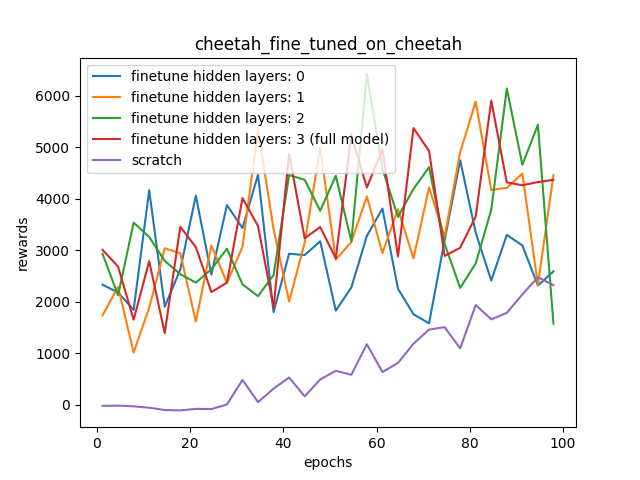
\includegraphics[width=0.6\textwidth]{../cache/pt/outputs/cheetah_fine_tuned_on_cheetah.png}}\end{subfigure}
    \begin{subfigure}[]{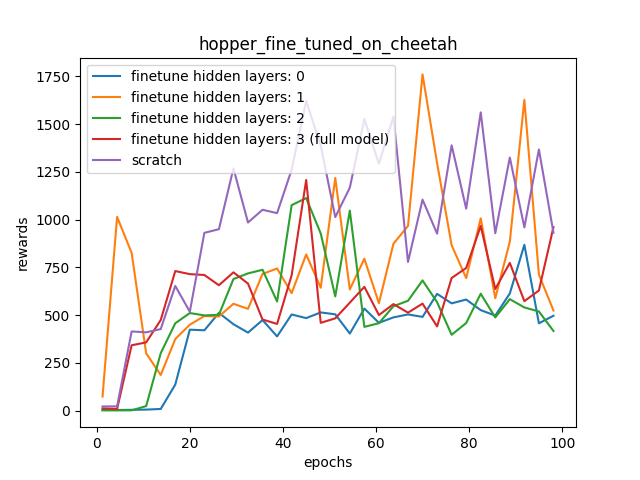
\includegraphics[width=0.6\textwidth]{../cache/pt/outputs/hopper_fine_tuned_on_cheetah.png}}\end{subfigure}
    \begin{subfigure}[]{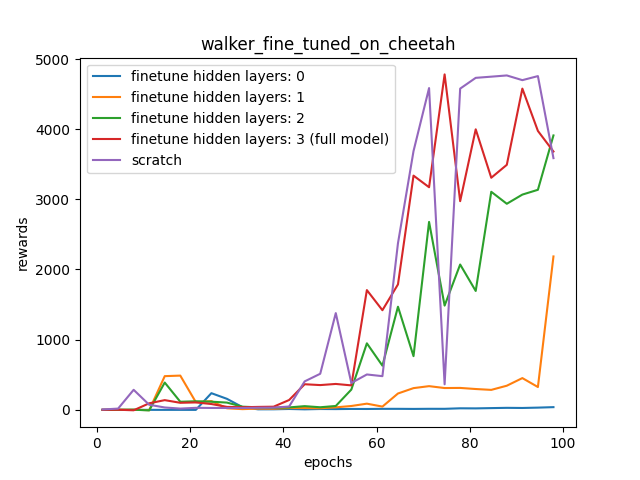
\includegraphics[width=0.6\textwidth]{../cache/pt/outputs/walker_fine_tuned_on_cheetah.png}}\end{subfigure}
    \caption{Target env: (a) Half-Cheetah, (b) Hopper, and (c) Walker2d all fine-tuned on source env: Half-Cheetah}
    \label{fig:x}
\end{figure*}
\begin{figure*}
    \centering
    \begin{subfigure}[]{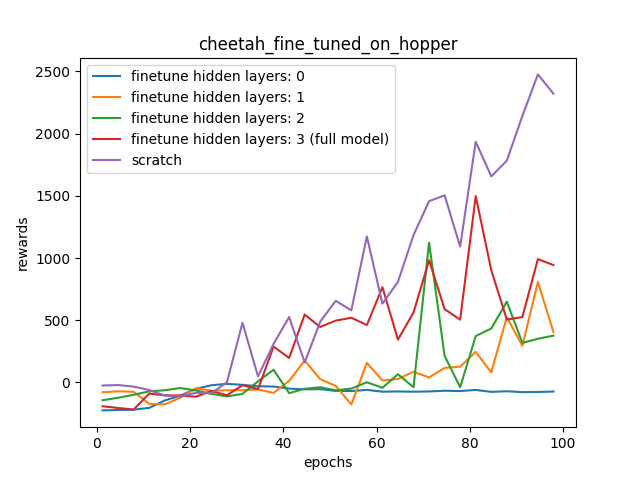
\includegraphics[width=0.6\textwidth]{../cache/pt/outputs/cheetah_fine_tuned_on_hopper.png}}\end{subfigure}
    \begin{subfigure}[]{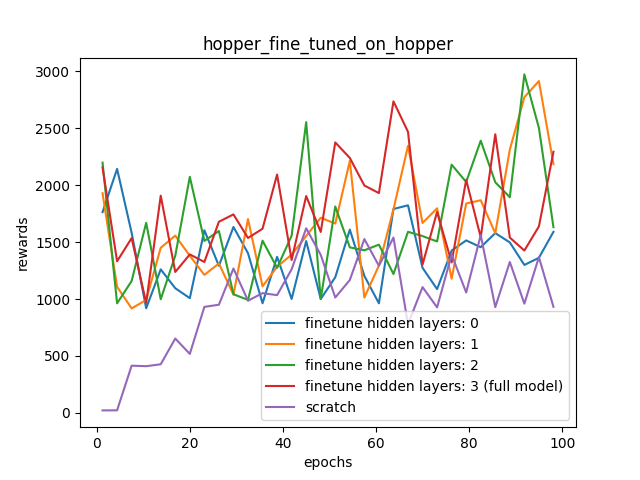
\includegraphics[width=0.6\textwidth]{../cache/pt/outputs/hopper_fine_tuned_on_hopper.png}}\end{subfigure}
    \begin{subfigure}[]{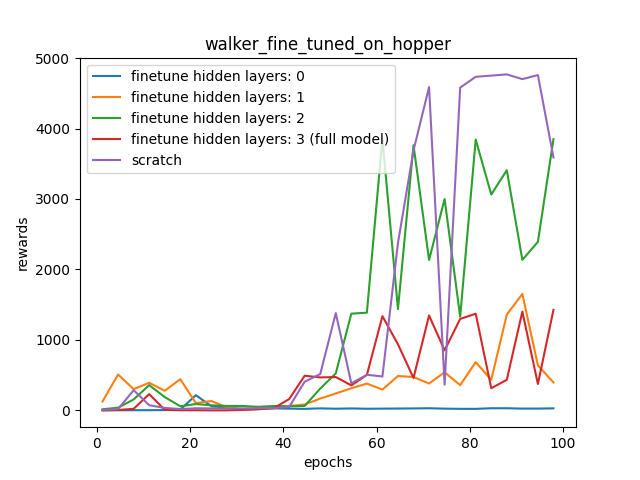
\includegraphics[width=0.6\textwidth]{../cache/pt/outputs/walker_fine_tuned_on_hopper.png}}\end{subfigure}
    \caption{Target env: (a) Half-Cheetah, (b) Hopper, and (c) Walker2d all fine-tuned on source env: Hopper}
    \label{fig:y}
\end{figure*}
\begin{figure*}
    \centering
    \begin{subfigure}[]{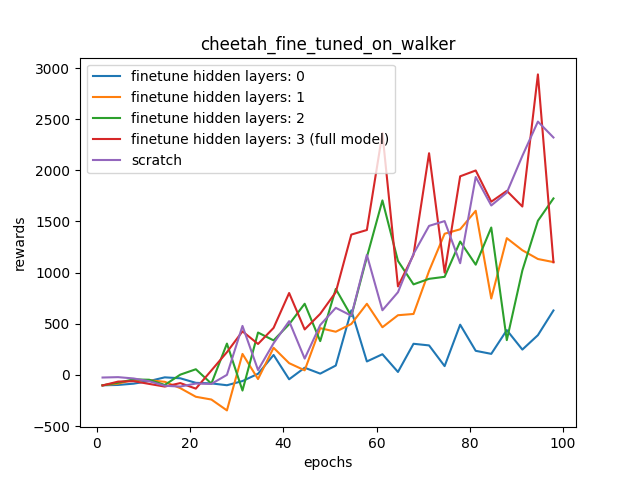
\includegraphics[width=0.6\textwidth]{../cache/pt/outputs/cheetah_fine_tuned_on_walker.png}}\end{subfigure}
    \begin{subfigure}[]{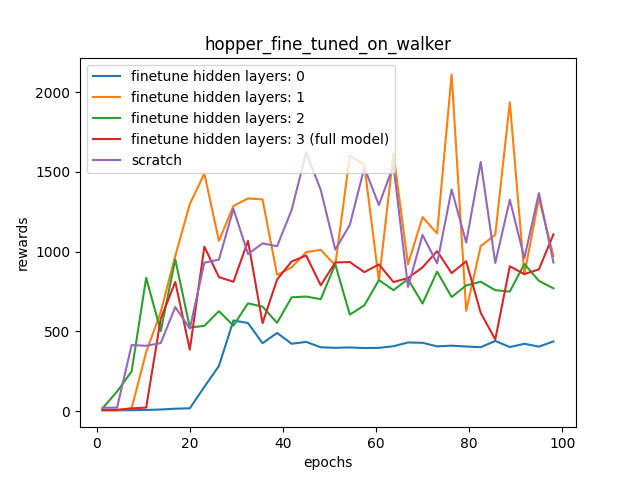
\includegraphics[width=0.6\textwidth]{../cache/pt/outputs/hopper_fine_tuned_on_walker.png}}\end{subfigure}
    \begin{subfigure}[]{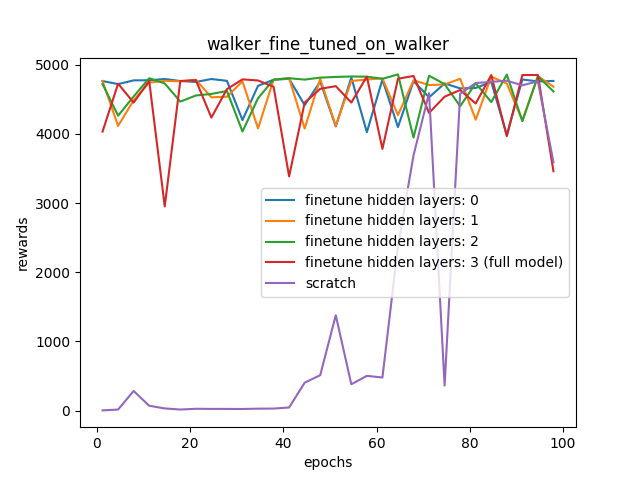
\includegraphics[width=0.6\textwidth]{../cache/pt/outputs/walker_fine_tuned_on_walker.png}}\end{subfigure}
    \caption{Target env: (a) Half-Cheetah, (b) Hopper, and (c) Walker2d all fine-tuned on source env: Walker2d}
    \label{fig:z}
\end{figure*}


\section{Conclusion and Future works}
In this project, I experimented with various fine-tuned policies in three environments to investigate whether fine-tuning would
impart an edge over the policies that are trained directly from scratch. The results indicate that this is possible for a certain combinations
of source and target environments. However, in the current experiments, the pre-trained policy was only trained on one source environment. In future,
I would like to experiment with the scenarios where the pre-trained policy is trained on multiple environments so as to learn from various tasks.
In such scenarios, fine-tuning over a new environment should provide more robust returns. Additionally, I would also like to experiment with
parameter-efficient ways for fine-tuning to investigate the minimum number of parameters that one might need to achieve the required returns.

\section{References}

\bibliographystyle{apalike}
\bibliography{naaclhlt2019}

\end{document}
